
%
% Chapter 6
%

\chapter{Future Work}

Throughout the course of this experiment, there have been a variety of areas that were adjusted to try and optimize the data. In this chapter, continued work and optimizations for future experiments are discussed.

\section{Detector Upgrades}

In a given experiment, the detectors are one of the single most important pieces of equipment. Two different styles of HPGe detectors were used, to varying success, and different magnetic configurations were used to optimize efficiency, discussed in Section \ref{sec:mini_orange}. Further steps are being taken for the future of conversion electron experiments at Notre Dame in both areas to improve the quality of data.

\subsection{fIREBAll}

The La Crosse \textbf{I}nternal Conve\textbf{R}sion \textbf{E}lectron \textbf{B}all \textbf{A}rray (fIREBAll) will be the next generation of ICEBall\citep{lesher19:_fireball}. The Major Research Instrumentation (MRI) proposal to the National Science Foundation (NSF) for funding has been approved. The University of Wisconsin-La Crosse submitted the proposal. The ICEBall beamline at the NSL will become the fIREBAll beamline. The focus of the proposal was detector upgrades, both for the Si(Li) detectors, and the HPGe detectors.

With this proposal, there will be dedicated HPGe detectors for the array, with two Bizmuth Germanate (BGO) anti-Compton suppression shields. The current Si(Li) detectors would be replaced with two Si(Li) detectors, for a total of twelve detectors each. There would still be six detection planes, as the Si(Li) detectors would be stacked in a telescope formation, to allow for the measurement of higher energy conversion electron transitions, including E0 transitions. The current Si(Li) detectors in use are 5 mm thick. All of the new detectors would be 5 mm thick, making for an active stopping depth of 10 mm when stacked. Additionally, the detectors would be 800 mm$^2$ surface area instead of 750 mm$^2$ of the current detectors. Over the past 25 years of use, the current Si(Li) detectors have begun to deteriorate. As seen in Figure \ref{fig:bad_sili}, there is a clear decline in the resolution of the detector between the different experiments.

\begin{figure}[!]
    \centering
    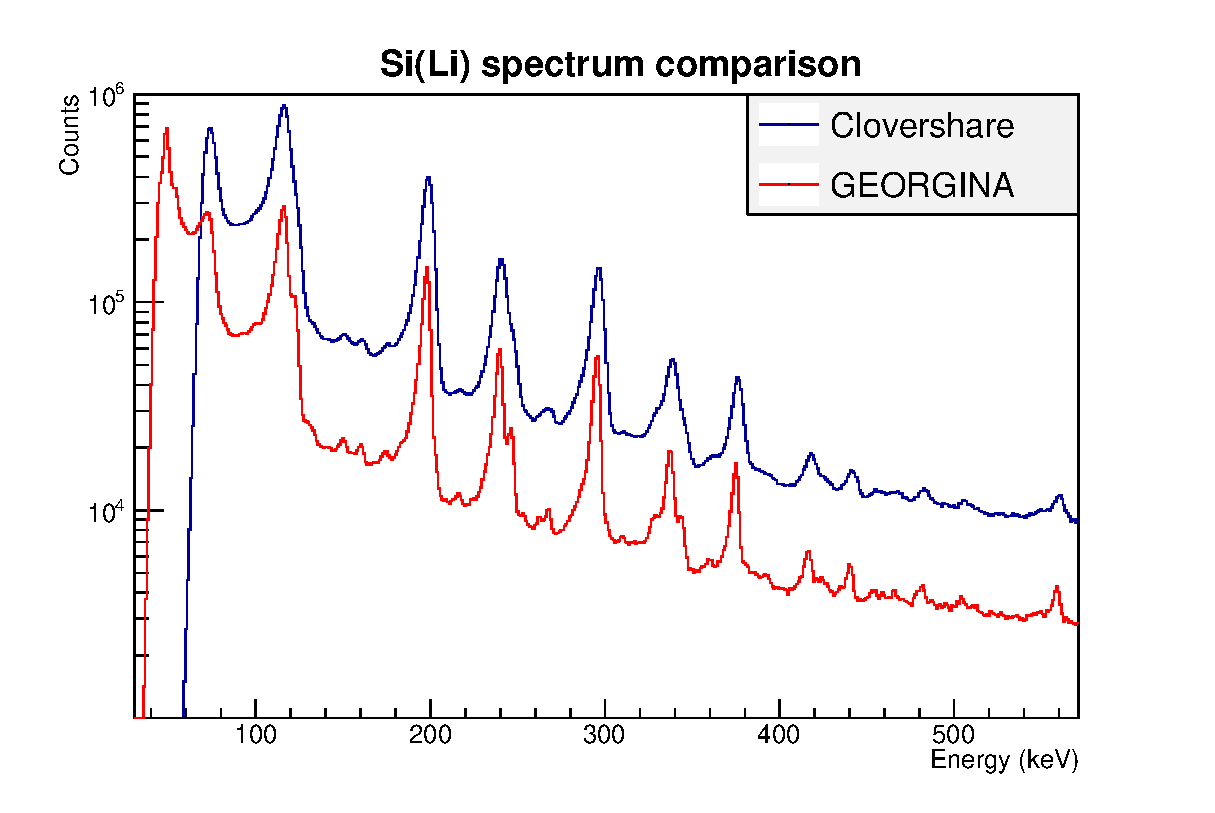
\includegraphics[scale=0.6]{Future_Figs/ResolutionComparison.eps}
    \caption{A comparison of the singles spectrum of one Si(Li) detector between the GEORGINA and Clovershare experiments. The resolution of the Si(Li) detector has deteriorated between the two experiments (the GEORGINA one was performed first). The LM peaks at \~{}240 keV and \~{}330 keV show this most clearly. The peaks are distinguishable in the GEORGINA data, but not in the Clovershare data.}
    \label{fig:bad_sili}
\end{figure}

\subsection{Magnet Designs}

To improve the detection efficiency of the conversion electrons, the magnetic configurations can be changed. This was done in the experiments to optimize for higher energies. When the experiments in this work were performed, the permanent magnets used were $36\times36\times5$ mm SmCo$_5$ squares. These thin squares are not, necessarily, creating the most optimal magnetic field.

Using GEANT4 and COMSOL, a variety of magnetic shapes were modeled, varying the cross-shape profile, the thickness, and the number of magnets used \citep{allison16:_geant4,comsol:_comsol}. Figure \ref{fig:fieldmap} shows what the magnetic fields look like when modelled in COMSOL. This figure is of the original magnets used in this work. Efficiencies of the new shapes were modeled from 0.1 to 1.0 MeV. The magnets were assumed to have a maximal side length of 37 mm. All of the magnets simulated were assumed to be Neodymium, specifically $\text{Nd}_{2}\text{Fe}_{14}\text{B}$.  In all of the shape testing, the number of magnets was varied to find idealized scenarios, with the magnets symmetrically spaced. The first variation was the cross-shape profile. Two extremes would be chosen, with intermediate steps between the extremes modelled and tested, as shown in Figure \ref{fig:cross-shape-slide}. Several hybrids of the intermediate steps were also examined, seen in Figure \ref{fig:cross_shape_hybrid}. the number of magnets was varied from 3 to 6 for each design, and evenly spaced.

\begin{figure}
    \centering
    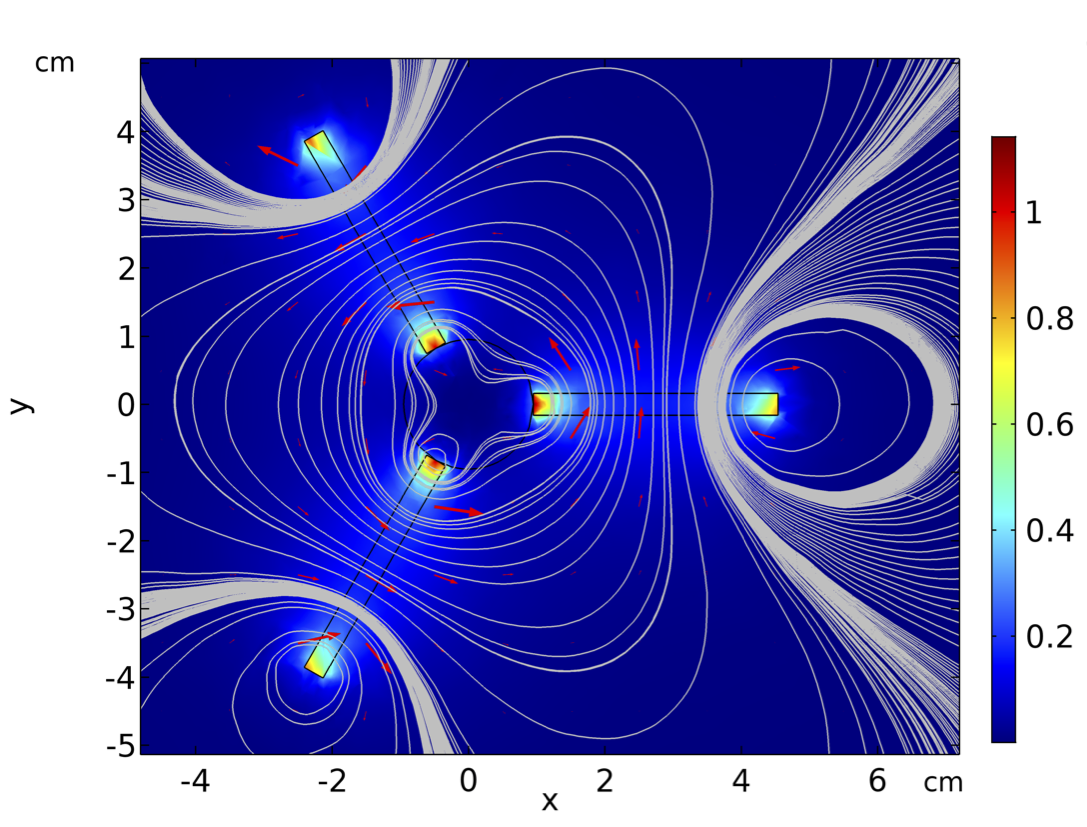
\includegraphics[scale=0.5]{Future_Figs/fieldmap.png}
    \caption{Map of the magnetic field lines, created through the use of COMSOL, for the original magnetic design \citep{comsol:_comsol}.}
    \label{fig:fieldmap}
\end{figure}

\begin{figure}
    \centering
    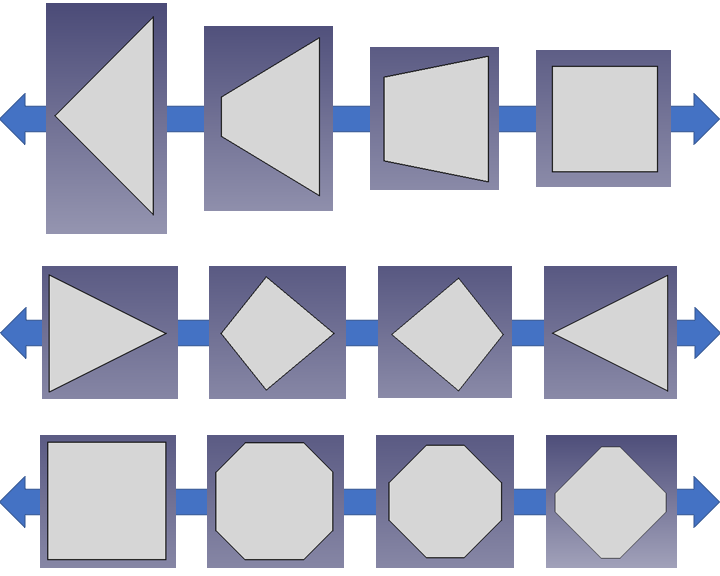
\includegraphics[scale=0.8]{Future_Figs/Cross-Shape-Slide.png}
    \caption{Initial tests of the cross shapes. The left-side of the shape would be the side against the blocker. Two extremes were chosen, with intermediate steps being tested between the two. These are the three sets of extremes used: large triangle to square, triangle with the base against the blocker to triangle with the point against the blocker, and square to truncated diamond.}
    \label{fig:cross-shape-slide}
\end{figure}

\begin{figure}
    \centering
    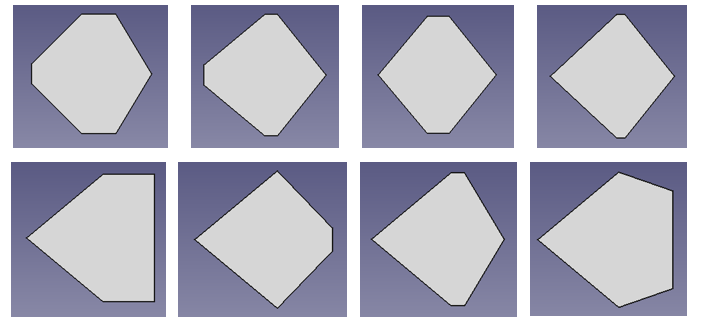
\includegraphics[scale=0.8]{Future_Figs/Cross-Shape-Hybrid.png}
    \caption{Sampling of the different hybrid cross shapes tested while examining magnetic designs. The left side of the shape would be the side against the central blocker.}
    \label{fig:cross_shape_hybrid}
\end{figure}

After picking the best cross-shapes, the thickness was varied between uniform and a gradient. Initially, this was a linear, uniform gradient. As simulations continued, variations in the form of the gradient were tested, including a step function, and a piecewise linear design, seen in Figure \ref{fig:width_shape}. As with the cross-shape, the number of magnets was varied for each design, ranging from 3 to 6 magnets.

\begin{figure}
    \centering
    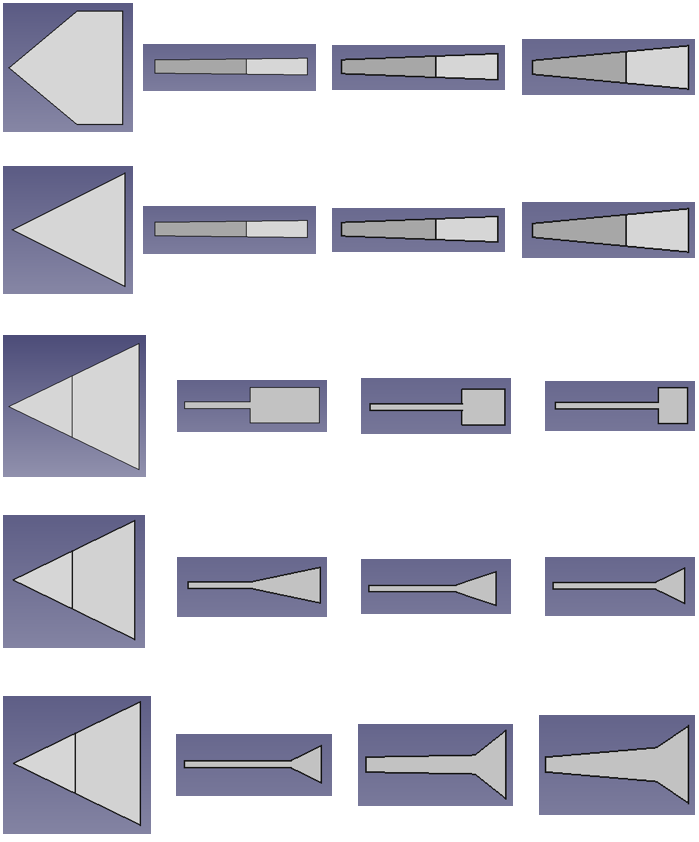
\includegraphics[scale=0.8]{Future_Figs/Width-Shape.png}
    \caption{Various width profiles tested for the magnets. The left figure shows the cross-shape for the width profiles. The left side goes against the central blocker. Variable gradients were looked at, starting with linear slopes, but evolving into step functions and piecewise linear slopes as the simulations expanded.}
    \label{fig:width_shape}
\end{figure}

Three designs were chosen after extensive simulations, to maximize efficiencies at low energies (0.2 to 0.4 MeV), high energies (0.7-1.0 MeV), and overall (0.2 to 1.0 MeV). This designs are shown in Figure \ref{fig:finalshapes} with simulated efficiencies for six magnet configurations. These designs have been ordered for testing with the detectors.

\begin{figure}
    \centering
    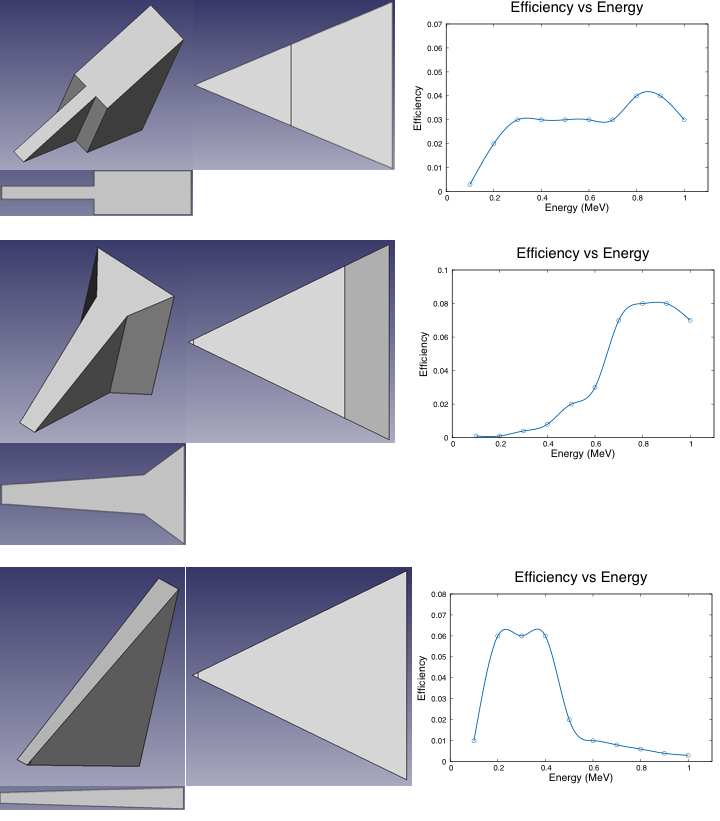
\includegraphics[scale=0.8]{Future_Figs/FinalShapes.png}  
    \caption{The final shapes chosen for testing. The left side goes against the central blocker. The top design has the best overall efficiency, the middle design has the best high energy efficiency, and the bottom design has the best low energy efficiency. These designs have been commissioned for testing.}
    \label{fig:finalshapes}
\end{figure}

\section{Target Upgrades}

One of the concerns and limitations of the original experiments was the thickness of the target. Ideally, the target being used would be less that 500 $\mu\text{g/cm}^2$, but the ones used were 1.7 $\text{mg/cm}^2$ and 1.44 $\text{mg/cm}^2$. While these targets were self-supporting, they were thick enough that electron straggling occurred, smearing out the spectrum.

To create a thinner target, it was decided to explore a carbon-backing. The Sm was evaporated onto a backing 20 $\mu\text{g/cm}^2$ thick. In the targets made, the Sm was measured to be 170 $\mu\text{g/cm}^2$, ten times thinner than the original targets used.

To compare the old and new targets, an experiment was run with both targets inside of ICEBall. The data compared was taken with the same electronics (discussed in the next section) and setup, to minimize differences that could impact the data.

The new targets could be run with higher beam currents to get similar rates in the detectors, at what appeared to be a proportional rate to the target thickness. At lower electron energies, the carbon-backed targets had far better resolution, as seen in Figure \ref{fig:target_test}. The centroids of the peaks also shifted in comparison between the thick and thin target, which follows logically from the thicker target causing greater energy loss. 

Also of note in Figure \ref{fig:target_test}, the thin target appears to have a higher background, causing the signal-to-noise ratio to decrease. To understand this increase in background, the beam was cut off and a new run was taken. Figure \ref{fig:O15decay} shows the detector trigger rate with respect to time during this background run. The background appears to show an exponential decay with a half-life on the order of two minutes.

\begin{figure}
    \centering
    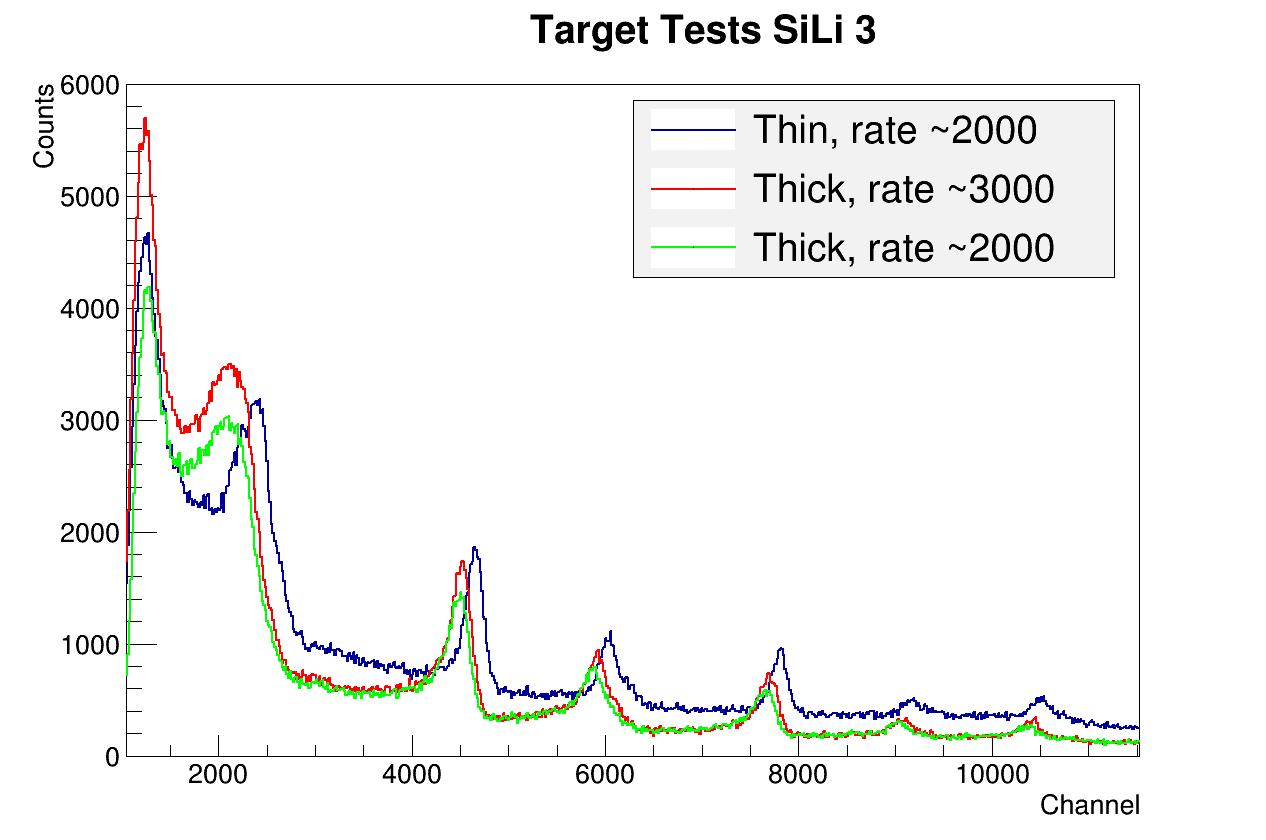
\includegraphics[scale=0.3]{Future_Figs/SiLi3.png}
    \caption{Comparison of the thick (self-supporting) and thin (carbon-backed) targets. The spectra were taken during the same experiment. At low energies, the resolution is better in the thin target. Further, the energies of the peaks shift based on which target it is. This spectrum is not energy calibrated.}
    \label{fig:target_test}
\end{figure}

\begin{figure}[!]
    \centering
    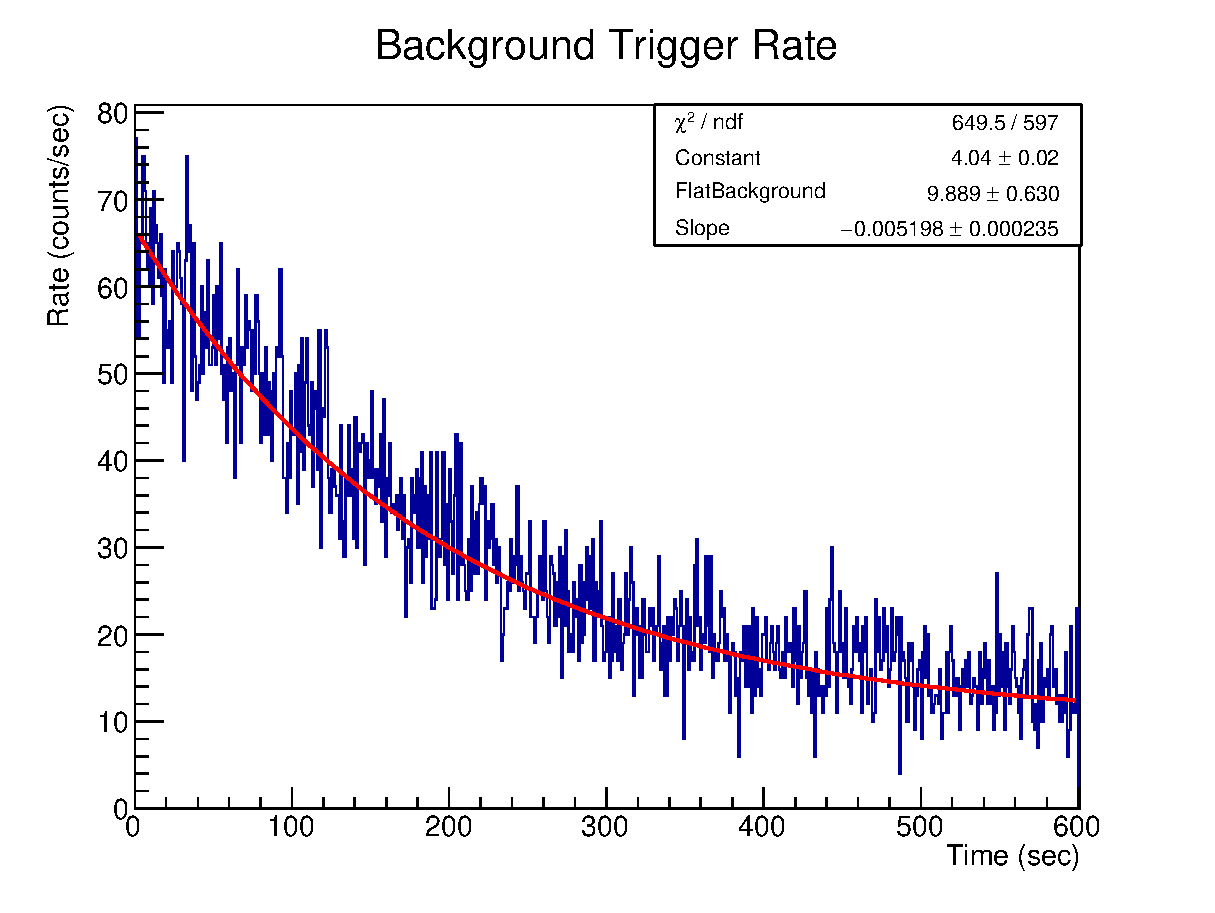
\includegraphics[scale=0.7]{Future_Figs/trigger_005.eps}
    \caption{Trigger rate of the background with respect to time, after running on one of the carbon-backed targets. There is a clear indication of an exponential decay, shown by the fit. The slope corresponds to a half-life of 133(5) seconds. $^{15}$O has a half-life of 122 seconds, within an acceptable error with the low statistics of the run.}
    \label{fig:O15decay}
\end{figure}

It was theorized this decay may be from $^{15}$O, which would be created from the $^{12}$C($\alpha,n$) reaction. Using the cross section, obtained from the EXFOR database, the cross section for this reaction at 20 MeV was obtained \citep{zerkin18:_exfor,black69:_carbonalphan}. This was used to calculate the rate in the detectors if it was $^{15}$O being created. These values matched, providing evidence of the new background element. One way this background can be decreased is by using thinner carbon-backing, as 12 $\mu g/cm^2$ is commercially available. This should reduce the $^{15}$O contribution the background by 40 percent.

\section{Electronics}

After experiments with two different electronics set ups, a third electronics set up was used, with the plan for it to become the standard electronics for future fIREBALL experiments. These electronics use the Mesytec MDPP-16 VME module and the Mesytec MVME data acquisition software \citep{mesytec:_mdpp,mesytec:_mvme}. The MVME software from Mesytec has built-in online analysis tools, allowing for real time analysis of the data and can be used with multiple types of VMEs. The MDPP-16 modules replace the conventional NIM modules, replacing external CFDs and TDCs. The gain, threshold, shaping time, and signal rise and decay times are all set within the module. 

The MDPP-16 modules can be run in multiple modes, depending on the firmware: QDC, SCP, and RCP modes. The firmware can be changed using a switch on the module, allowing a given module to hold all three firmware versions. For these tests, the SCP, or standard charge sensitive preamplifier, mode is used. Figure \ref{fig:mdpp_schematic} shows the schematic configuration of the module in SCP mode, and Table \ref{tab:word_MDPP} shows the breakdown of the event words in the system.

\begin{figure}[!t]
    \centering
    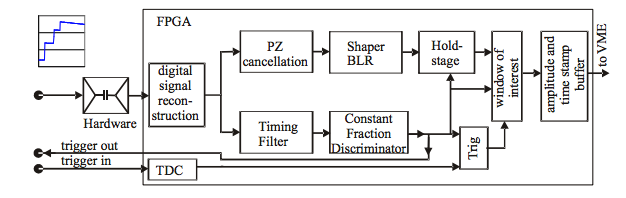
\includegraphics[scale=0.65]{Future_Figs/MDPP_Schematic.png}
    \caption{A schematic representation of the MDPP-16 software in SCP mode. The amplitude and timing are separated out into individual signals. Signal properties, shaping time, and the threshold can all be adjusted. Taken from \citep{mesytec:_mdpp}.}
    \label{fig:mdpp_schematic}
\end{figure}

One of the benefits of the MDPP-16 modules is the compatibility with other VME modules. Scaler values can be read in with a separate module, such as the CAEN V830, as was done with the GEORGINA setup, discussed in Section \ref{sec:GEORGINA_electronics}. Many of the scaler values can be read in using the MDPP-16, but the addition of the V830 allows for more versatility in rates to record, including comparing rates between the MDPP-16 and the V830 for deadtime corrections.

\section{Outlook}

Testing with the new magnetic configurations is currently underway, while the new detectors are being manufactured. The electronics have been tested and used extensively at the NSL. Future experiments with the new fIREBall system will have greater sensitivity, contributing to the effort to probe the nuclear chart for E0 transitions in the search for understanding collective modes and shape coexistence.

\begin{landscape}
    \begin{table}[]
    \footnotesize
    \centering
    \caption{\label{tab:word_MDPP}Data Event - MDPP-16 (32 Bit Word)}
    \begin{tabular}{c|c|c|c|c|c|c|c|c|c|c|c|c|c|c|c|c|c|c|c|c|c|c|c|c|c|c|c|c|c|c|c}
        \toprule
        \multicolumn{32}{c}{Header} \\
        \hline
        \multicolumn{2}{c|}{2} & \multicolumn{2}{|c|}{2} & \multicolumn{4}{|c|}{4} & \multicolumn{8}{|c|}{8} & \multicolumn{3}{|c|}{3} & \multicolumn{3}{|c|}{3} & \multicolumn{10}{|c}{10} \\
        \addlinespace[-2ex]
        \multicolumn{2}{c|}{header} & \multicolumn{2}{|c|}{subheader} & \multicolumn{4}{|c|}{} & \multicolumn{8}{|c|}{module id} & \multicolumn{3}{|c|}{TDC} & \multicolumn{3}{|c|}{ADC} & \multicolumn{10}{|c}{number of} \\
        \addlinespace[-2ex]
        \multicolumn{2}{c|}{signature} & \multicolumn{2}{|c|}{} & \multicolumn{4}{|c|}{} & \multicolumn{8}{|c|}{} & \multicolumn{3}{|c|}{\_resolution} & \multicolumn{3}{|c|}{\_resolution} & \multicolumn{10}{|c}{following words} \\
        \hline
        \multicolumn{2}{c|}{b01} & \multicolumn{2}{|c|}{b00} & \multicolumn{4}{|c|}{xxxx} & \multicolumn{8}{|c|}{module id} & \multicolumn{3}{|c|}{bxxx} & \multicolumn{3}{|c|}{bxxx} & \multicolumn{10}{|c}{number of 32} \\
        \addlinespace[-2ex]
        \multicolumn{2}{c|}{} & \multicolumn{2}{|c|}{} & \multicolumn{4}{|c|}{} & \multicolumn{8}{|c|}{} & \multicolumn{3}{|c|}{} & \multicolumn{3}{|c|}{} & \multicolumn{10}{|c}{bit data words} \\
        \midrule
        \multicolumn{32}{c}{Data Word} \\
        \hline
        \multicolumn{2}{c|}{2} & \multicolumn{2}{|c|}{2} & \multicolumn{4}{|c|}{4} & \multicolumn{2}{|c|}{2} & 1 & \multicolumn{5}{|c|}{5} & \multicolumn{16}{|c}{16}\\
        \addlinespace[-2ex]
        \multicolumn{2}{c|}{data-sig} & \multicolumn{2}{|c|}{} & \multicolumn{4}{|c|}{} & \multicolumn{2}{|c|}{} &  & \multicolumn{5}{|c|}{} & \multicolumn{16}{|c}{}\\
        \hline
        \multicolumn{2}{c|}{b00} & \multicolumn{2}{|c|}{01} & \multicolumn{4}{|c|}{xxxx} & \multicolumn{2}{|c|}{(pu,ov)} & Trigger Flag & \multicolumn{5}{|c|}{channel number} & \multicolumn{16}{|c}{ADC Value}\\
        \hline
        \multicolumn{2}{c|}{2} & \multicolumn{2}{|c|}{2} & \multicolumn{6}{|c|}{6} & 1 & \multicolumn{5}{|c|}{5} & \multicolumn{16}{|c}{16}\\
        \addlinespace[-2ex]
        \multicolumn{2}{c|}{data-sig} & \multicolumn{2}{|c|}{} & \multicolumn{6}{|c|}{} &  & \multicolumn{5}{|c|}{} & \multicolumn{16}{|c}{}\\
        \hline
        \multicolumn{2}{c|}{b00} & \multicolumn{2}{|c|}{01} & \multicolumn{6}{|c|}{xxxxxx} & Trigger Flag & \multicolumn{5}{|c|}{channel number + 16} & \multicolumn{16}{|c}{TDC time difference}\\
        \midrule
        \multicolumn{32}{c}{End of Event} \\
        \hline
        \multicolumn{2}{c|}{2} & \multicolumn{30}{|c}{30}\\
        \hline
        \multicolumn{2}{c|}{b11} & \multicolumn{30}{|c}{Event counter/time stamp}\\
        \bottomrule
    \end{tabular}
    \\[2pt]
    \footnotesize
    Table of the 32-bit word data structures of the Mesytec MDPP-16 in the SCP Firmware. The headers, event word structure, and end of event structure, where needed, are all listed. In the tables, the first row in a given block is the number of bits used by that piece of data, while the second row is a description of the data. Bits go in descending order from left to right. Data has two words, one for the amplitude and one for the corresponding timing. The (pu,ov) bits are for pile up, underflow, and overflow flags.
\end{table}
\end{landscape}
